\documentclass[journal]{IEEEtran}
\usepackage[utf8]{inputenc}
\usepackage{amsmath}
\usepackage{amssymb}
\usepackage{textcomp,gensymb}
\usepackage{hyperref}
\hypersetup{
    colorlinks = true,
    urlcolor = blue,
    citecolor = black,
    linkcolor = black
} 
\usepackage[bottom=2cm, right=3cm, left=3cm, top=1.5cm]{geometry}
\usepackage{cancel}
\usepackage{physics}
\usepackage{booktabs}
\usepackage{graphicx}
\graphicspath{ {./images/} }
%\begin{center}\includegraphics[scale = 0.25]{name}\end{center}
\newcommand{\R}{\mathbb{R}}
\newcommand{\Z}{\mathbb{Z}}
\newcommand{\qed}{\qquad${}$\hfill$\square$\\}
\newcommand{\qqR}{\qquad\Rightarrow\qquad}
\newcommand{\qqand}{\qquad\text{and}\qquad}
\newcommand{\qqor}{\qquad\text{or}\qquad}
\newcommand{\qiff}{\quad\Longleftrightarrow\quad}
\newcommand{\qqiff}{\qquad\Longleftrightarrow\qquad}
\newcommand{\qqiffdf}{\qquad\Longleftrightarrow_{df}\qquad}
\renewcommand{\b}[1]{\boldsymbol{#1}}

\usepackage{todonotes}

\begin{document}

\title{Three Competing Models for Superpredator Release}

\author{Group~11:
    Kevin~Hefner,
    Shri~Lekkala,
    and YingTing~Lu}
    
\markboth{STAT 37830: Scientific Computing with Python - Final Report. December 8th, 2023.}{Kevin Hefner, Shri Lekkala, and YingTing Lu}

\maketitle

% 1. An introduction to the topic of your project. Cite any resources that contribute to your discussion.
% Include why we have 3 models
% Don't include equations
% "spatially homogenized model"
% Introduce cane toad analogue
\section{Introduction}
\IEEEPARstart{C}{omplex} ecosystems and precise inter-species dynamics can often be simplified to an elementary food web, delineating predators and their prey. To understand how populations of different animals ebb and flow through seasons and habitat changes, conservationists and biologists model population growth and decay with computer simulation.\par
This project serves as a breadth-before-depth look at three contrasting approaching to modeling the predator-dynamics that arise when we introduce a superpredator, a third animal that preys on all others, to a living environment \cite{cats_protecting_birds, cats_protecting_revisited}.\par
The scientific interest in this ``superpredator release" arises in situations where new species are introduced to control existing species, and when invasive species spread through delicate ecosystems \cite{invasive_species}. In northern Australia, the introduction of the invasive cane toad (\emph{Rhinella marina}) has been linked to decreases in monitor lizard populations, and increases the populations of the monitors' prey population \cite{Invasive_toads}.\par
As with most complex processes that would be intractable to model to extreme accuracy, each possible models highlights some features and ignores others. We have thus created three specialized models of this superpredator release, so that each has advantages and weaknesses depending on implementation.\par
First, we created a model that utilizes an ordinary differential equation (ODE), specifically the Lotka-Volterra equations \cite{meiss_textbook}. These equations simply model how population counts influence other population counts, with no focus on individual animal-interactions.\par
Next, we have a spatially-homogenized agent model. Here, we represent each animal individually, and at each discrete timestep, all animals have an equal probability of interaction. This attributes more weight and control over how the animals hunt, in comparison to the ODE model above.\par
Finally, we extended the previous model to create a spatial agent model. Again, interactions between animals are computed individually, but now almost all effort is weighted into the spatial aspects. Animals are only able to interact with those around them.\par
As we discuss each of these models, we will gain a perspective of how a scientist should choose a model for their specific requirements and restrictions. It is not our goal to equate the behavior produced by each model, but instead to appreciate their differences.

% 2. An introduction to the numerical methods or packages that you will use in your project, and the notation you will use. Cite any resources that contribute to your discussion. Note that this needs to be detailed enough for someone not knowledgeable in your topic to replicate your results.
% clarify that ODE solution is concatenated
% clarify 3rd species introduction
% Explain interaction of agents
% OOP is independent of complexity of numerical method
% Explain all notation (including subscripts)
\section{Numerical Methods, Packages, and Notation}
In all three models, we use \verb|numpy| to store information in arrays, as well as for the typical array-manipulating methods. We also use \verb|matplotlib.pyplot| for plotting.\par
In all models, we are modeling the same type of superpredator release. In the middle of our simulation time frame, we instantaneously release a population of the superpredators, where there is no initial population of this species. For simplicity, these superpredators are assumed to be introduced all at the same time, so there is no ``ramp-up" of population, just a instant step to the released population.\par
There is randomness present in the spatially homogenized and spatial agent model, and in order for simulations to be repeatable, we ``seed" the random number generators depending on the sum of all initial populations, so that two trials, even with different probabilistic parameters or numbers of iterations, are given the same random generation when starting with the same populations.\par
Continuing, our three models have varied implementations, so we discuss each individually.
\subsection{The Differential Equation Model}
The standard differential equation used for modeling predator-prey situations is the Lotka-Volterra equations \cite{meiss_textbook}. We have generalized these equations to instead model dynamics between three species, where $A$ represents the prey, $B$ represents the predators, and $C$ the superpredators.
$$\begin{cases}
    \dv{A}{t} = r_0A\qty(1-\frac{A}{K}) - \mu_0AB - \nu_0AC\\
    \dv{B}{t} = -r_1B + \mu_1AB - \eta_0BC\\
    \dv{C}{t} = -r_2C + \nu_1AC + \eta_1BC
\end{cases}$$
There are many terms here, so we will explain the notation used for each. $r_0,r_1,r_2$ are the absolute growth rates, where $r_0$ is the uninhibited growth of the prey, and $r_1,r_2$ are the death rates of the predators and superpredators respectively. $K$ signifies the carrying capacity of the environment, i.e. the maximum number of prey animals that can exist before they begin to die, as if by overpopulation. $\mu_0$ and $\mu_1$ model the predators hunting prey, where $\mu_0$ is the rate at which prey are hunted, and $\mu_1$ is the rate at which predators can be born due to the gained food by hunting. Variables $\nu_0$ and $\nu_1$ similarly model the superpredators hunting prey, with the same usages as for $\mu_0,\mu_1$. Finally, $\eta_0$ and $\eta_1$ model the superpredators hunting predators.\par
In order to numerically solve this ODE with superpredator release, we concatenate two solutions to the Lotka-Volterra equations above. First, we use \verb|scipy.integrate.solve_ivp| to numerically estimate the solution for the time up until the superpredators are released. We then modify the final position of this solution to add the superpredator population. Then, using this modified final state as the initial condition, we again run the ODE solver to compute behavior from the release time to the end of our simulation time span. The concatenated output of both calls to \verb|solve_ivp| gives all information needed, and thus this ODE model is complete.

\subsection{The Spatially Homogenized Agent Model}
Our spatially homogenized agent model is discrete, as opposed to the continuous ODE model above; we iterate through time steps that could be analogous to ``days" of our simulation. This model used creates a class \verb|Nonspatial_Agent| that allows for simpler implementation of interactions between agents \cite{Agents.jl,Goodwill}. The main interest of this model is that we also consider the health of each animal, mostly based on food availability. Each day, the agent loses one ``health point", which can only be replenished by feeding on a successful hunt.\par
In each iteration of this model, we model reproducing and hunting for each species. We loop through a list of agents of each species. First the agent loses one health-point, if they live through this (i.e. have more than 1 health-point remaining), we randomly determine if that agent will reproduce in this iteration. We finally model hunting, where predators and superpredators have a parameterized probability of successful hunting, and get the chance to hunt each possible prey agent, all with equal probability of success.\par
There are some notable details of this iteration process. We must allow superpredators to hunt both predator and prey agents. We additionally consider a parameter giving the carrying capacity as before, where we give a bonus reproduction-chance when the population of prey is below the carrying capacity. To conclude one iteration, we drop all agents that have died during this day, and append the newly birthed agents.\par
Finally, while there is no notation used in this model, we can discuss the available arguments with which one can tune the simulation. Most arguments with the same effect are passed as a list, with each element applying to one species. The user can determine the initial health of a newly birthed animal with \verb|init_health|, and set the carrying capacity with the aptly named \verb|carrying_capacity_A|. Most interactions are determined by given probabilities, where \verb|hunt_success_probs| gives the probability of the predator and superpredator killing a given target, and \verb|reproduction_probs| gives the probability of each species reproducing each iteration. Finally we can set the gained health-points from killing a given species using \verb|food_values|.

\subsection{The Spatial Agent Model}
To create a spatial agent model, we move our focus from the individual agents, as in the spatially homogenized agent model, to the physical positioning and spatial behaviors of the agents. We have removed the health-point feature from our previous model, so that we can better focus on the spatial aspects here. Thus, we no longer need lists of agent objects, and instead use a 2D-array, which holds integers to signify which agent (or lack of an agent) is located in each cell of our grid of positions. We then simulate interactions on this grid.\par
As we iterate through ``days" similarly to the spatially homogenized model, we simulate interactions between cells, using a scheme that generalizes Conway's Game of Life \cite{game_of_life}. The user can give arguments to set the minimum and maximum number of neighbors for the survival of a cell, and the exact number of neighbors required for a new agent to be born. As a holdover from the spatially homogenized model, we have more parameters for the probability that a cell is successful in hunting one of its neighbors. This highlights a key difference in the agent-to-agent interactions in this model. Agents are only able to interact with the 8 (or fewer) neighbors, and this requires that all of the interactions as we loop though cells of our grid are proceeding by identifying the list of agents for a given cell.\par
Notably, this model also uses the \verb|matplotlib.animation.FuncAnimation| class, to create \verb|.gif| files that animate the physical state of our simulation as we iterate. These animations allow the user to gain perspective on how the chosen parameters effect the spatial aspects of our simulation which is the key differential between this model and others.\par
One more interesting feature of this model is way in which the initial populations of each species are added to the grid. Instead of randomly placing agents into empty cells, we instead generate ``blobs" of agents of the same species that grow until we have initialized the correct number of agents. These blobs are grown by randomly adding agents around one ``seed" cell, with a small probability to move this seed to an adjacent cell. Once a cell has all filled neighbors, the seed is randomly moved to begin generating a new blob.

% 3. A brief description of how you are structuring the Python package src and a description of your main functions.
% explain (in not to much detail) what functions are needed to run the models
\section{Structure of src Folder}
We have three models, each with its own contained behavior and methods, and we will be writing each model as a class. When the user instantiates an instance of that class, the model is constructed and finishes all computations at initialization. The directory \verb|src\| contains one \verb|.py| file for each model. Making each model its own file in \verb|\src| allows for code to be constructed and modified without affecting other models, and keeps all functions needed for one model in one file for readability.\par
There are two more files present in the \verb|\src\| folder: \verb|tools.py|, which contains some common functions used to validate inputs; and \verb|__init__.py| which exists to define the variable \verb|__all__|, so that \verb|import *| works as intended.\par
In order to run the models, only access to the three model classes are required (\verb|ODE_Superpredator_Release|, \verb|Nonspatial_Agent_Model|, and \verb|Spatial_Agent_Model|). The user creates the model by constructing a object of the chosen class with the required parameters. From here, the user has a few options to access the information resulting from their simulation.\par
All models can produce a simple \verb|PyPlot| of the populations over time with the \verb|.plot()| function. The user can retrieve a useful output explaining the chosen arguments with the property \verb|.arguments|, and get a list of the minimum and maximum populations of each species using \verb|.get_population_extremes()|. Finally, the spatial agent model has a special method, \verb|.save_gif()| that saves an animated GIF of the grid of agents over time to a given filename.\par
There are a few more methods that have less common uses that are included, such as \verb|.equation_string| for the ODE model, and additionally methods are not useful to a scientist interested in using these simulations, and those are thus omitted here.

% 4. A description of what tests are in test.
% Give more description than given in the Midterm report
\section{Tests and Code Validation}
Within the test directory, there are four test files that test each of the files in the \verb|\src\| directory. The tests are built using the python unittest framework and they run from the test directory by using the command \verb|pytest|. Across the four test files there are 69 unittests which all pass.

The unit tests are broadly split into two categories: input validation tests, and functionality tests.
In \verb|test_ode_model.py|, \verb|test_spatial_agent_model.py| and \verb|test_nonspatial_agent_model.py|, all the input validation unit test cases are contained within the class \verb|TestInvalidInputs|. For each possible user inputted parameter of the model, these tests check that an invalid input is correctly identified and the corresponding error is raised with the appropriate error message. For example, within the file \verb|nonspatial_agent_model.py|, in the class \verb|Nonspatial_Agent_Model|, there are input validation checks (in the form of property attributes for each user defined parameter of the class) which ensure that an error is raised if the input is not as expected. In particular, for the parameter \verb|N_release|, it checks that this variable is an integer, and is between 0 and \verb|n_steps|. Now within the test file, the function \verb|test_N_release| tries invalid inputs for \verb|N_release|, and checks that the relevant exception is caught and raised for each one. The advantage of input validation is that if a user incorrectly or unknowingly inputs an invalid value, then they will know exactly what to modify in order to get the model working as expected.

Additionally, in each of the test files, there are functionality tests that are responsible for testing that each individual function works as expected. The test classes that contain all such unit tests are \verb|TestODESuperpredatorRelease|, \verb|TestNonspatialAgent|, \verb|TestNonspatialAgentModel|, \verb|TestSpatialAgentModelFunctions|, \verb|TestNeighborsFunction|, and \verb|TestIsANumber|. 
For example, the function \verb|test_iteration| in \verb|TestSpatialAgentModelFunctions| sets the spatial grid to a predetermined initialization, runs one iteration using the \verb|.iteration| method, checks the result is what we expect, and then runs further iterations to check that the final grid is what is expected. It should be noted that both the Spatial and Nonspatial Agent model are non-deterministic as they involve random initializations and probabilities. However, this issue can be avoided when testing by fixing a random seed, and also using probabilities of 1 or 0 in the parameters of the model so we know with certainty what the behavior of the model should be.

Overall, the unit tests in the test suite cover a wide range of scenarios including testing invalid inputs, individual functions, individual agent behaviors, and overall model dynamics.


% 5. Report on your investigations into the effectiveness of your method. Remember that our main focus is on scientific computing, so try to look into the accuracy/efficiency of your methods and/or the efficiency of your code.
% Bring up cane toad analogue again
% Clarify which parameters are changed at each model
% "Explore how the time step affects the discrete model"
% Compare the models

\newpage

\section{Our Investigations and Evaluating Our Models}
\subsection{Model Differences}

% \begin{table*}[t]
% \centering
% \begin{tabular}{|p{1.6cm}|p{3.2cm}|p{3.2cm}|p{3.2cm}|}
% \hline
% \textbf{Aspect} & \textbf{ODE Model (Lotka-Volterra Equations)} & \textbf{Homogeneous Agent-Based Model} & \textbf{Spatial Agent-Based Model} \\ \hline
% Population Dynamics & Yes & Yes & Yes \\ \hline
% Individual-Level Interactions & No & Yes & Yes \\ \hline
% Spatial Considerations & No & No & Yes \\ \hline
% Animal Representation & Aggregate populations & \raggedright Individual agents& Individual agents \\ \hline
% Habitat Structure & Not considered & Not considered & Considered \\ \hline
% Interaction Probabilities & Not applicable & Equal for all agents & Spatially dependent \\ \hline
% \end{tabular}
% \vspace{2mm}
% \caption{Comparison of three models}
% \label{tab:comparison}
% \end{table*}

In this project, we set out to create 3 vastly different models of predator-prey dynamics under a superpredator release situation. The parameters used in such models are difficult if not impossible to measure in the real-world, since our models are greatly simplified and combine multiple behaviors into the same parameter. Thus, the \emph{effectiveness} of our models is instead a measure of the ability of each model to give unique results. There is no ``ground truth" to which we compare these models, and thus we instead consider the issues when using the models without a wider context beyond an interest in the models themselves. These three models have different focuses. Let us examine each one separately: \par
\subsubsection{ODE Model (Lotka-Volterra Equations)}
This is the basic model, considering only the overall impact among different populations. It involves parameters related to growth rates, death rates, carrying capacity, hunting rates and reproduction rates. These differential equations capture the large-scale dynamics of overpopulation and hunting, but fails to capture any granular actions of individual animals.\par
Since all parameters of this model are free to be decimals, there is a great deal of flexibility. The user can tune the rate at which one species is hunted by another, and independently tune how much the predator population increases from this hunting.\par
Based on our experience in creating the examples found later in this paper, the ODE model is the easiest to manipulate into specific behavior, as there is an almost infinite parameter-space of options to choose when instantiating a model.

\subsubsection{Spatially Homogenized Agent Model}
In this model, individual interactions in terms of hunting behavior are emphasized. New parameters, such as health points and time steps, are introduced to simulate the condition and temporal relationships of individual animals being preyed upon.\par
Using probabilities to define many of the interactions allows for a great deal of freedom, but now that populations are fixed to be integers, some parameters, such as \verb|food_values| and \verb|init_healths| must also be integers. As a result, changing these integers parameters by only one, the smallest possible step, can have significant changes in long-term behavior, without the ability for further tuning.\par
However, one must appreciate that this spatially homogenized model also captures important biological constants that are lost in the ODE model. Most importantly, the timescale of this model is more accurate, as the user can determine the initial health, and thus minimum lifespans, of the agents. The Lotka-Volterra equations above can have unnatural spikes downwards, often due to uncontrolled population growth, but this is inaccurate. In real ecosystems, a large spike in predators would most likely cause extinction of the prey, which is modeled correctly in both models, but this would then be followed by a slow starvation of the predators.\par
Our spatially homogenized agent model strikes a fair midpoint between the flexibility of the ODE model while still considering important features such as lifespan, without the restrictions present in the Spatial Agent Model.

\subsubsection{Spatial Agent Model}
The focus here shifts from individual agents to their physical positions and spatial behaviors. Compared to the homogenized agent model, parameters related to health points are removed. Instead, hunting success probabilities and geographic positions (whether another agent is in the surrounding 8 positions) are adjusted to simulate predation situations. Similar to the homogenized model, iteration steps are used to model the temporal relationships of individual animals being preyed upon.\par
Most noticeably in this model, the minimum population for survival, the overpopulation threshold, and the breeding population requirements all must be integers. Only considering the eight neighbors, all of these values be between zero and eight, heavily restricting the model's outcomes.\par
The set of possible simulations is thus smaller than in the other models, but this is somewhat remedied by the ability to select the grid-size. Smaller grids are more prone to complete extinction, while large grids with small initial populations often result in a lack of any inter-species interactions. This is as desired however, as this model's focus, to the detriment of other features, is the spatial characteristics of a simulation.\par
A scientist interested in superpredator over-hunting for example, may wish to use a different model. A different scientist with a focus on ecosystems restricted to say, a small island, would be far more interested in this model, as spatial consequences of a restricted space will be more influential.

\vspace{-3mm}
\begin{table}[b]
\begin{tabular}{|p{1.5cm}|p{1.5cm}|p{1.5cm}|p{1.5cm}|}
\hline
\textbf{Aspect}               & \textbf{ODE Model (Lotka-Volterra Equations)} & \textbf{Spatially Homogenized Agent Model} & \textbf{Spatial Agent Model} \\ \hline
Population Dynamics           & Yes                                           & Yes                                        & Yes                          \\ \hline
Individual-Level Interactions & No                                            & Yes                                        & Yes                          \\ \hline
Spatial Considerations        & No                                            & Yes                                        & Yes                          \\ \hline
Animal Representation         & Aggregate populations                         & Individual agents                          & Individual agents            \\ \hline
Habitat Structure             & Not considered                                & Not considered                             & Considered                   \\ \hline
Interaction Probabilities     & Not applicable                                & Equal for all agents                       & Spatially dependent          \\ \hline
\end{tabular}
\vspace{0.1mm}
\caption{Comparison of three models}
\label{tab:comparison}
\end{table}

\newpage

\subsection{Parallel Simulations with Similar Parameters}
We strive to use (nearly) identical parameters for initial setup and compare the results of the three models, for four archetypal environmental changes after superpredator release.\par
In each model, shared parameters will be kept constant or proportional, but clearly those parameters that are unique to one model must be chosen anew. While some parameters have weakly related pairings across models, we do not attempt to relate them. This section instead serves as a proof of concept of the flexibility of each model, and to demonstrate their function to model the same outcomes, and not the same inputs (due to the incongruence of parameters).\par
Please see the Appendix for parameters chosen in each model. Additionally, if you wish to see any of the animations created by the Spatial Agent Model, please find them in the Github \href{https://github.com/UChi-ComPy23/group-project-group_11/tree/main/examples}{here}.

\subsubsection{Inconsequential Superpredator Release}
In this section, we model a situation in which the superpredators are not suited for long-term survival in the new ecosystem they are released into. Thus, we selected parameters such that the superpredators die out quickly, without changing any of the long-term behavior of the prey and predator populations.\par
We initialize all models with 50 prey, 10 predators, and we release 5 predators halfway through a 50 time-unit simulation.\par
One crucial feature of our models, as shown in Figures \ref{fig:inconsequential_superpredator_release_ode},\ref{fig:inconsequential_superpredator_release_nonspatial}, and \ref{fig:inconsequential_superpredator_release_spatial} is the carrying capacity. We can see that the prey population always reaches some maximum and stays near that maximum.
In both the ODE and Spatially Homogenized Agent Model, we have set the environmental carrying capacity for species A, causing this limit to their population. When exceeded, we model some form of overcrowding we causes a population decrease. This is directly implemented in the first two models, but exists in the spatial model due to the \verb|maximum_counts| parameter, after species $A$ (the prey) has covered a proportion of the entire grid.\par
In this example, from the graph of the ODE Model, we observe that species A and B had already reached equilibrium with a significant difference in population before the release of species C. Therefore, although the release briefly causes a decrease in the population of species B (with a corresponding increase in species A), it eventually returns to a certain balance. On the other hand, the Spatial Agent Model shows somewhat similar results to other models, where all three species eventually reach equilibrium. However, the population of species A increases compared to the initial state. The inference drawn here could be due to the different method of controlling the population of species A in this model, which takes into account the spatial factor. Hence, when species are dispersed, the limiting effect on species quantity tends to be slower in this model.

\begin{figure}[h]
    \vspace{-4mm}
    \centering
    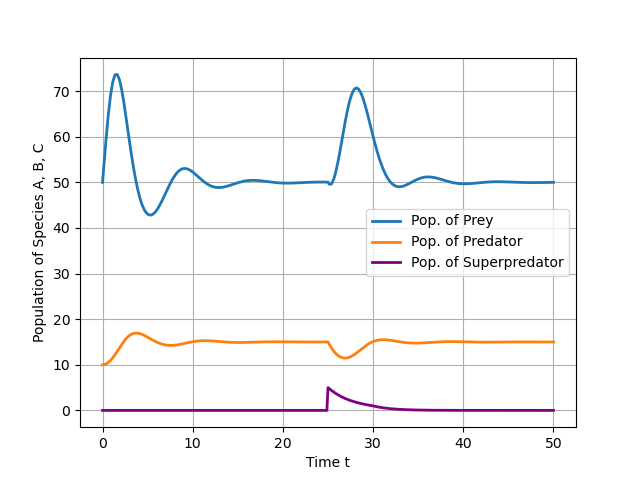
\includegraphics[width=8cm]{images/inconsequential_superpredator_release_ode.png}
    \vspace{-8mm}
    \caption{ODE Model's Inconsequential Superpredator Release}
    \label{fig:inconsequential_superpredator_release_ode}
\end{figure}
\begin{figure}[h]
    \vspace{-8mm}
    \centering
    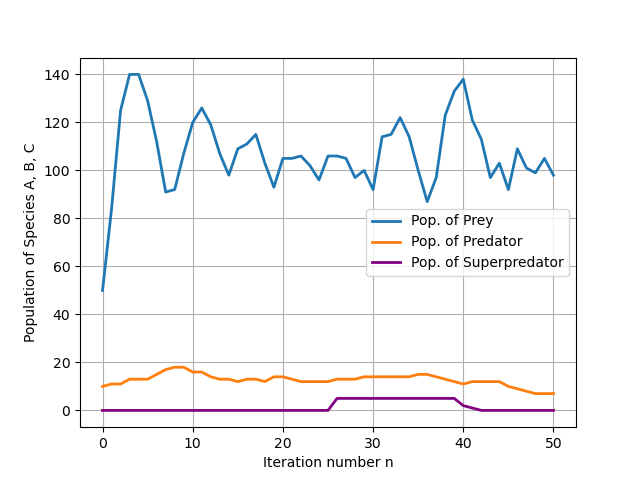
\includegraphics[width=8cm]{images/inconsequential_superpredator_release_nonspatial.png}
    \vspace{-8mm}
    \caption{Nonspatial Model's Inconsequential Superpredator Release}
    \label{fig:inconsequential_superpredator_release_nonspatial}
\end{figure}
\begin{figure}[h]
    \vspace{-8mm}
    \centering
    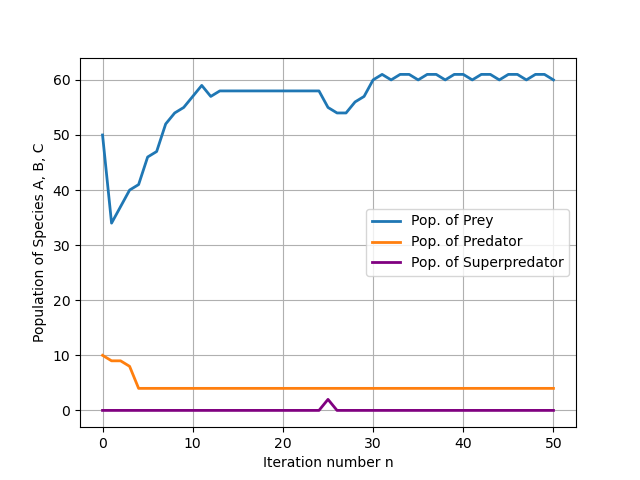
\includegraphics[width=8cm]{images/inconsequential_superpredator_release_spatial.png}
    \vspace{-8mm}
    \caption{Spatial Model's Inconsequential Superpredator Release}
    \label{fig:inconsequential_superpredator_release_spatial}
\end{figure}


\subsubsection{Mesopredator Replacement}
Our next situation of interest is one of mesopredator replacement. In the ``middle"-predator (mesopredator) dies out after the introduction of the new superpredator.\par
This is most easily achieved in our models by making the predator species have a weak population, that is heavily preyed upon by the superpredators.\par
In each of the models' simulations in Figures \ref{fig:mesopredator_replacement_ode}, \ref{fig:mesopredator_replacement_nonspatial}, and \ref{fig:mesopredator_replacement_spatial}, we can see that some equilibrium is reached between the prey and predators before the superpredators' release. When the invasive superpredators are introduced, their predation of the of the mesopredators causes the mesopredator extinction, while the superpredators gain an ecological niche in the long-term.\par
We can see that in the ODE and Spatial Agent Models, this replacement of one predator for another causes a new equilibrium to be found, in which the prey population is higher than previously observed. In the Spatially Homogenized Agent Model, we have that the prey population is most limited by the environmental carrying capacity, before and after mesopredator replacement.

\begin{figure}[h]
    \vspace{-5mm}
    \centering
    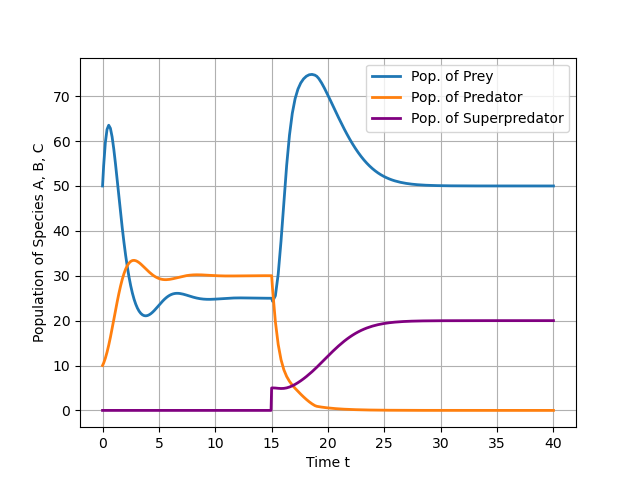
\includegraphics[width=7.5cm]{images/mesopredator_replacement_ode.png}
    \vspace{-8mm}
    \caption{ODE Model's Mesopredator Replacement}
    \label{fig:mesopredator_replacement_ode}
\end{figure}
\begin{figure}[h]
    \vspace{-7mm}
    \centering
    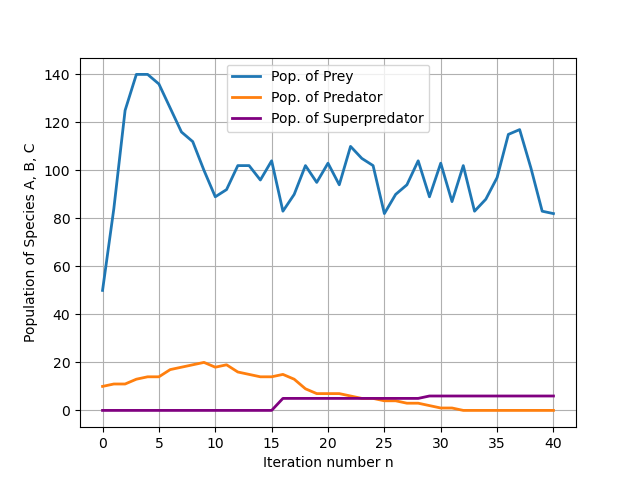
\includegraphics[width=7.5cm]{images/mesopredator_replacement_nonspatial.png}
    \vspace{-8mm}
    \caption{Nonspatial Model's Mesopredator Replacement}
    \label{fig:mesopredator_replacement_nonspatial}
\end{figure}
\begin{figure}[h]
    \vspace{-7mm}
    \centering
    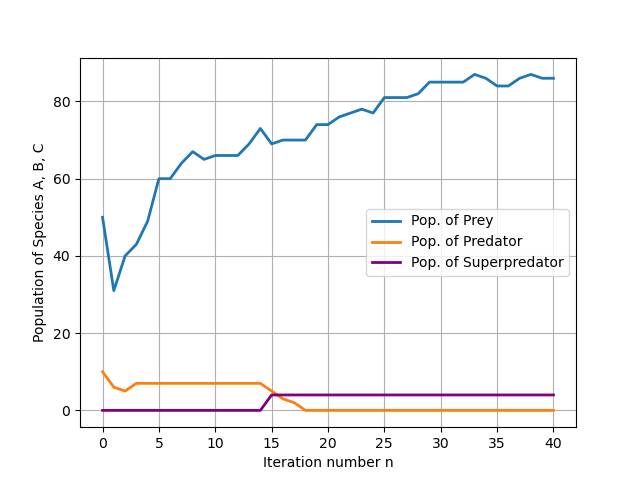
\includegraphics[width=7.5cm]{images/mesopredator_replacement_spatial.png}
    \vspace{-8mm}
    \caption{Spatial Model's Mesopredator Replacement}
    \label{fig:mesopredator_replacement_spatial}
\end{figure}

\newpage

\subsubsection{Catastrophic Release}
Now consider the terrible situation in which a food web is so weak that the superpredators are able to destabilize the entire system, leading to the eventual extinction of all species.\par
We have tuned parameters in each of our models so that this is accomplished through a ``population explosion" in the superpredators. The superpredator populations, increasing greatly from their release-population, grow to a point that is not sustainable by the environment. In this case, the superpredators overfeed on both types of prey, causing their extinction. As the simulation progresses, the superpredators also become extinct due to lack of food.\par
The Spatial Agent Model was the most resistant to modeling this outcome in our study, as the spatial restrictions of agents often results in small ``stable pockets" of only a few individuals. As we have not modeled any wandering of agents throughout the grid, these pockets never interact, and true extinction is thus unlikely. Thus, in our spatial simulation, Figure \ref{fig:catastrophic_release_spatial}, we see that Species A and C do not go fully extinct, but continue at greatly reduced populations from initial values.

\begin{figure}[h]
    \vspace{-4mm}
    \centering
    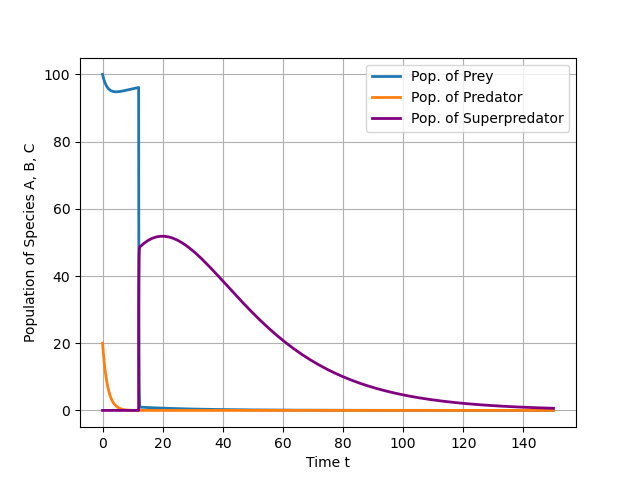
\includegraphics[width=8cm]{images/catastrophic_release_ode.png}
    \vspace{-8mm}
    \caption{ODE Model's Catastrophic Release}
    \label{fig:catastrophic_release_ode}
\end{figure}
\begin{figure}[h]
    \vspace{-5mm}
    \centering
    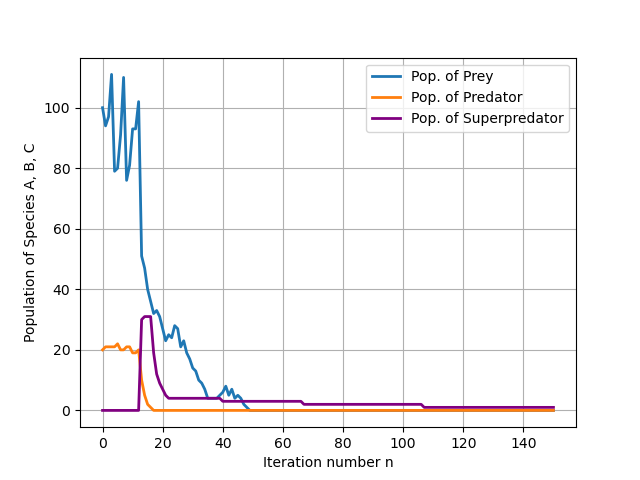
\includegraphics[width=8cm]{images/catastrophic_release_nonspatial.png}
    \vspace{-8mm}
    \caption{Nonspatial Model's Catastrophic Release}
    \label{fig:catastrophic_release_nonspatial}
\end{figure}
\begin{figure}[h]
    \vspace{-5mm}
    \centering
    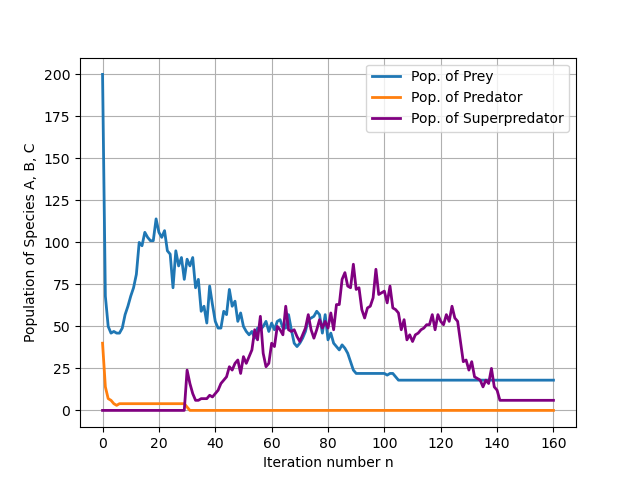
\includegraphics[width=8cm]{images/catastrophic_release_spatial.png}
    \vspace{-8mm}
    \caption{Spatial Model's Catastrophic Release}
    \label{fig:catastrophic_release_spatial}
\end{figure}

\newpage

\subsubsection{Superpredator Harmony}
Our final example is the most applicable to ecology and invasive species today. Here, we select parameters so that the superpredators are able to thrive in their new environment, but in a controlled way in which no other species go extinct. As with the mesopredator release situation, the long-term equilibrium found after this release may change, but we expect all species to be resistant to extinction.\par
This example draws intriguing parallels with the documented ecological shifts resulting from the invasive cane toads in Australia \cite{Invasive_toads}. In this real-world scenario, the invasive cane toad (superpredator) led to severe population declines in three species of predatory monitor lizards (predators), namely the yellow-spotted monitor, Mertens’ water monitor, and Mitchell’s water monitor. These declines, amounting to approximately 50\% over a five-year period, were caused by toad-induced lethal toxic ingestion and triggered cascading effects on the prey species, exemplified by the Crimson Finch. The Crimson Finch experienced a notable increase in fledging success from 55\% to 81\% in response to the reduced predation pressure from the declining water monitor populations \cite{Invasive_toads}. The modeled superpredator, thriving in a controlled manner, resonates with the invasive cane toad situation by showcasing a scenario where careful management allows the survival of all species without facing extinction.\par

%%  May be unnecessary:
% This parallelism underscores the intricate dynamics of predator–prey relationships, highlighting the need for comprehensive understanding and effective management to mitigate the ecological impacts of invasive species and sustain a harmonious balance in natural ecosystems.

Now looking at our results (Figures \ref{fig:superpredator_harmony_ode}, \ref{fig:superpredator_harmony_nonspatial}, and \ref{fig:superpredator_harmony_spatial}), we can see that each model has features that are unlike the previous examples. The ODE Model exemplifies the new equilibrium that can be created. Before the superpredator introduction, the population of the predators was quite high, and prey very low, but this becomes inverted in the new paradigm. We can also see that the oscillations that are visible at times before superpredator released are damped-out after release.\par
Contrast this with the Spatially Homogenized model, in which oscillations are maintained throughout the entire timescale. We can see that the prey population stays high near the environmental carrying capacity, but there is clear competition between predators and superpredators as they form peaks and valleys in opposite phase.\par
Finally, in the spatial agent model, we see that not all species must be influenced by new introductions. The mesopredator population is almost constant throughout, and only the prey population decreases as superpredators find their niche.

\begin{figure}[h]
    \vspace{-5mm}
    \centering
    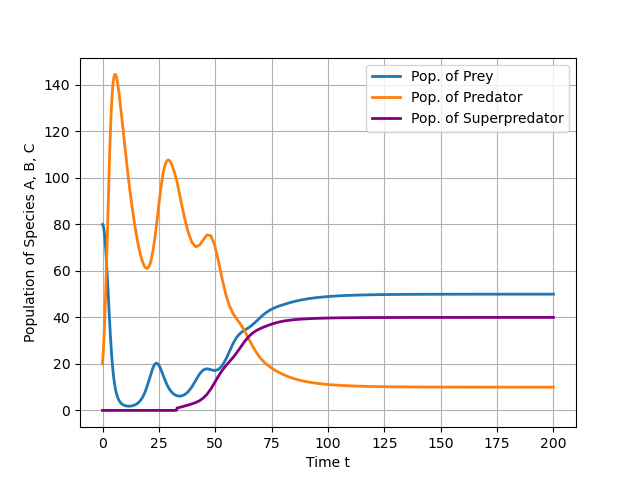
\includegraphics[width=8cm]{images/superpredator_harmony_ode.png}
    \vspace{-8mm}
    \caption{ODE Model's Superpredator Harmony}
    \label{fig:superpredator_harmony_ode}
\end{figure}
\begin{figure}[h]
    \vspace{-5mm}
    \centering
    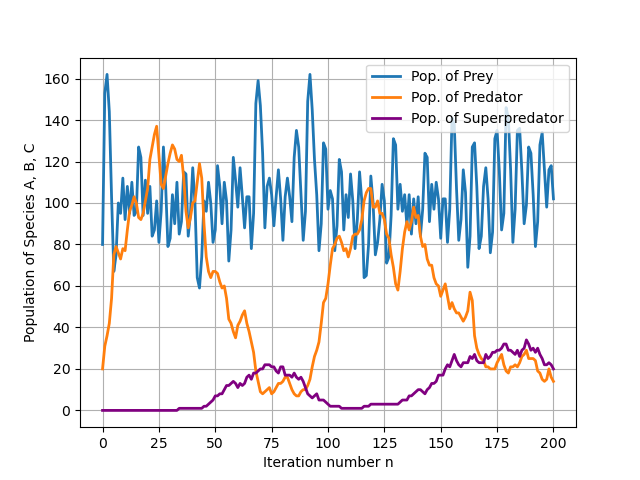
\includegraphics[width=8cm]{images/superpredator_harmony_nonspatial.png}
    \vspace{-8mm}
    \caption{Nonspatial Model's Superpredator Harmony}
    \label{fig:superpredator_harmony_nonspatial}
\end{figure}
\begin{figure}[h]
    \vspace{-5mm}
    \centering
    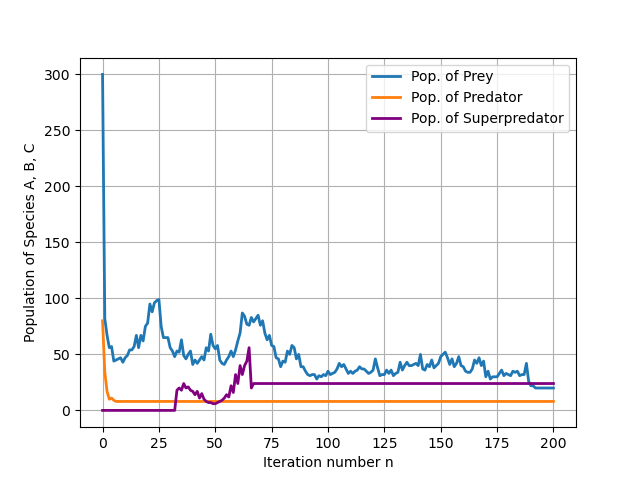
\includegraphics[width=8cm]{images/superpredator_harmony_spatial.png}
    \vspace{-8mm}
    \caption{Spatial Model's Superpredator Harmony}
    \label{fig:superpredator_harmony_spatial}
\end{figure}

\newpage

\subsection{Timing Comparison}
Interested in the speed of these competing models, we have performed a simple timing experiment. We have computed the runtime of each model 25 times, beginning at model instantiation and ending when the simulation terminates. We have selected the same parameters as the Superpredator Harmony Example above, to avoid models becoming trivially simple due to extinction before simulation termination. For the ODE Model and Spatially Homogenized Model, this is simply timing the object constructors, but for the Spatial Agent Model, we must also save the animation to a \verb|.gif| file, as this function call is the point at which all iterations run. Each model has been run with a time parameter of 200, i.e. 200 seconds for the ODE solver, and 200 iterations in the agent models.\par
Based on the results in Table \ref{model_runtimes}, we have found that as expected, the ODE Model is the fastest, taking an average of 7 milliseconds to complete one simulation. The Spatially Homogenized model is the second fastest, taking approximately 20$\times$ as long (140 milliseconds on average), and the Spatial model is by far the slowest (9.5 seconds on average). This extreme slowdown is likely due to the overhead of creating and saving the animation to a \verb|.gif| file, as the other simulations lack this requirement.
\begin{table}[h]
\caption{Comparison of Model Runtimes, (seconds)}
\label{model_runtimes}
\begin{tabular}{lrrr}
\toprule
 & $\mqty{\text{ODE}\\\text{Model}}$ & $\mqty{\text{Nonspatial}\\\text{Agent Model}}$ & $\mqty{\text{Spatial}\\\text{Agent Model}}$ \\
\midrule
mean & 0.007596 & 0.143722 & 9.560396 \\
std & 0.001022 & 0.002850 & 0.318636 \\
min & 0.006837 & 0.138431 & 9.324225 \\
50\% & 0.007349 & 0.142846 & 9.421552 \\
max & 0.012162 & 0.149366 & 10.771482 \\
\bottomrule
\end{tabular}
\end{table}


\newpage

\section*{Contributions}
\subsubsection*{Kevin Hefner} Coded the methods in \verb|ODE_Model|, \verb|Nonspatial_Agent|, \verb|Nonspatial_Agent_Model|, and \verb|Spatial_Agent_Model| used for simulation. Coded \verb|.plot()| for each method. Created Jupyter notebooks for examples 1-4 and for timing comparison. Wrote final report sections I, II and V; and assisted with section III. Wrote analysis for example 2, example 3, and timing comparison. Contributed to analysis for examples 1 and 4. Formatted LaTeX document.

\subsubsection*{Shri Lekkala} Coded input validation checks for each method, and coded  all 4 unit-testing files \verb|/test/|. Wrote final report section III and IV, and contributed to analysis for example 4.

\subsubsection*{YingTing Lu} Coded \verb|arguments| and \verb |get_population_extremes| for each method. Wrote final report section V and analysis for example 1.

\bibliographystyle{plain}
\bibliography{Bibliography.bib}

\newpage

\section{Appendix}
\subsection{Inconsequential Superpredator Release Parameters}
\subsubsection{ODE Model}
\begin{verbatim}
r = [2, 0.5, 0.5]
K = 200
mu = [0.1, 0.01]
nu = [0.02, 0.002]
eta = [0.05, 0.004]
t_bounds = [0, 50]
A0 = 50
B0 = 10
T_release = 25
C_T = 5
\end{verbatim}
\subsubsection{Spatially Homogenized Agent Model}
\begin{verbatim}
init_healths = [3, 10, 15]
hunt_success_probs = [0.0025, 0.00]
food_values = [2, 5]
reproduction_probs = [0.40, 0.05, 0]
carrying_capacity_A = 100
A0 = 50
B0 = 10
N_release = 25
C_N = 5
n_steps = 50
\end{verbatim}
\subsubsection{Spatial Agent Model}
\begin{verbatim}
breeding_counts = [3, 3, 4]
minimum_counts = [2, 2, 3]
overpopulation_counts = [6, 4, 5]
hunt_success_probs = [1, 0.33]
A0 = 50
B0 = 10
N_release = 25
C_N = 4
n_steps = 50
m = 10
n = 10
\end{verbatim}

\subsection{Mesopredator Replacement Parameters}
\subsubsection{ODE Model}
\begin{verbatim}
r = [4, 0.5, 0.5]
K = 100
mu = [0.1, 0.02]
nu = [0.1, 0.01]
eta = [0.25, 0.01]
t_bounds = [0, 40]
A0 = 50
B0 = 10
T_release = 15
C_T = 5
\end{verbatim}
\subsubsection{Spatially Homogenized Agent Model}
\begin{verbatim}
init_healths = [3, 10, 15]
hunt_success_probs = [0.0025, 0.03]
food_values = [2, 5]
reproduction_probs = [0.40, 0.08, 0.02]
carrying_capacity_A = 100
A0 = 50
B0 = 10
N_release = 15
C_N = 5
n_steps = 40
\end{verbatim}
\subsubsection{Spatial Agent Model}
\begin{verbatim}
breeding_counts = [3, 3, 3]
minimum_counts = [2, 2, 3]
overpopulation_counts = [6, 4, 5]
hunt_success_probs = [1, 0.33]
A0 = 50
B0 = 10
N_release = 15
C_N = 5
n_steps = 40
m = 12
n = 12
\end{verbatim}

\subsection{Catastrophic Release Parameters}
\subsubsection{ODE Model}
\begin{verbatim}
r = [0.05, 0.7, 0.04]
K = 100
mu = [0.002, 0.001]
nu = [0.3, 0.06]
eta = [0.1, 0.02]
t_bounds = [0, 150]
A0 = 100
B0 = 20
T_release = 12
C_T = 30
\end{verbatim}
\subsubsection{Spatially Homogenized Agent Model}
\begin{verbatim}
init_healths = [2, 2, 5]
hunt_success_probs = [0.05, 0.5]
food_values = [1, 2]
reproduction_probs = [0.80, 0.02, 0.001]
carrying_capacity_A = 100
A0 = 100
B0 = 20
N_release = 12
C_N = 30
n_steps = 150
\end{verbatim}
\subsubsection{Spatial Agent Model}
\begin{verbatim}
breeding_counts = [3, 3, 3]
minimum_counts = [2, 2, 2]
overpopulation_counts = [4, 4, 4]
hunt_success_probs = [0.2, 0.3]
A0 = 200
B0 = 40
N_release = 30
C_N = 62
n_steps = 160
m = 40
n = 40
\end{verbatim}

\subsection{Superpredator Harmony Parameters}
\subsubsection{ODE Model}
\begin{verbatim}
r = [1, 0.1, 0.3]
K = 100
mu = [0.01, 0.01]
nu = [0.01, 0.005]
eta = [0.01, 0.005]
t_bounds = [0, 200]
A0 = 80
B0 = 20
T_release = 33
C_T = 1
\end{verbatim}
\subsubsection{Spatially Homogenized Agent Model}
\begin{verbatim}
init_healths = [2, 2, 5]
hunt_success_probs = [0.01, 0.005]
food_values = [1, 2]
reproduction_probs = [0.85, 0.51, 0.1]
carrying_capacity_A = 100
A0 = 80
B0 = 20
N_release = 33
C_N = 1
n_steps = 200
\end{verbatim}
\subsubsection{Spatial Agent Model}
\begin{verbatim}
breeding_counts = [3, 4, 3]
minimum_counts = [2, 2, 2]
overpopulation_counts = [4, 5, 4]
hunt_success_probs = [0.4, 0.7]
A0 = 300
B0 = 80
N_release = 33
C_N = 20
n_steps = 200
m = 35
n = 35
animation_length = 15
\end{verbatim}

\end{document}